Computer vision is an important and maturing engineering science. It underpins an increasing variety of applications that require the acquisition, analysis and interpretation of visual information.

\subsubsection{Feature extraction}
When working with images, it is usually not possible to work with the raw image data (the pixel values) due to its high dimensionality. 
By extracting features from images, they can be represented in a lower dimensional feature-space.  This feature extraction process has several advantages:
\begin{itemize}
\item The data becomes computationally easier to work with due to the lower dimensionality
\item By using appropriate features, the data becomes more suitable for generalization across images
\item Reducing the dimensionality makes it easier to visualize sets of images
\item Features can have an intuitive basis, which makes it easier for non-computer-scientists to analyze (sets of) images
\end{itemize}

In the extraction of image features, a distinction was made between low-level statistical features and higher level cognitive-based features.\\

\paragraph{\textit{Statistical features}}
Many relatively simple low-level statistical features were extracted from the images.
The first type of statistical features used are color-based features, which capture the color-usage in the artwork. Many artists produce collections of art pieces with similar colors, and should therefore be (partially) distinguishable using color-based features. For each of the three RGB channels, an average and median is calculated over all the channel values. Let $\{\mathbf{x}_{m,i,c} \}_{i=1\dots n}$ be the pixel values for image $m$ in color channel $c \in \{R,G,B \}$. The average in channel $c$ of image $m$ is given by: 

\begin{equation}
\label{avgChannel}
\mu_c(\mathbf{x}_{m}) = \frac{1}{n}\sum_{i=1}^{n} \mathbf{x}_{m,i,c} 
\end{equation}
The median in channel $c$ is given by 
\begin{equation}
\label{medChannel}
\tilde{\mathbf{x}}_{m,c} = \mathbf{x'}_{m,k,c}
\end{equation}
where $\{\mathbf{x'}_{m,i,c}\}_{i = 1\dots n}$ are the sorted pixel values of channel $c$ and $k = \mbox{round}(n/2)$.
The image is also converted into the HSV color space, from which the average and median is extracted for each channel as defined in equations \ref{avgChannel} and \ref{medChannel}. The Hue channel is given by: \\\\

$H_{m,i} = \left\{ 
\begin{array}{ll}
0 & \mbox{if $C_{m,i} = 0$};\\
60 \left(\frac{G_{m,i}-B_{m,i}}{C_{m,i}} \mbox{mod} 6 \right) & \mbox{if $M_{m,i} = R_{m,i}$};\\
60 \left(\frac{B_{m,i}-R_{m,i}}{C_{m,i}} + 2 \right) & \mbox{if $M_{m,i} = G_{m,i}$};\\
60 \left(\frac{R_{m,i}-G_{m,i}}{C_{m,i}} + 4 \right) & \mbox{if $M_{m,i} = B_{m,i}$}; \\
\end{array}
\right\}$\\\\

Where $M_{m,i} = \max(R_{m,i},G_{m,i},B_{m,i})$ and $C_{m,i} =  M - \min(R_{m,i},G_{m,i},B_{m,i})$. The value channel is given by $V_{m,i} =  M_{m,i}$ and the saturation channel is  by $S_{m,i} = \frac{C_{m,i}}{V_{m,i}}$

The second group of features is the edge to pixel and corner to pixel ratio. Let $\{\mathbf{x}_{m,i} \}_{i=1\dots n}$ be the pixel values of the binary edge-image produced by applying a Canny Edge detector \cite{cannyEdge} on image $m$. The edge to pixel ratio of image $m$ is then computed as $f_{e,m} = \frac{1}{n}\sum_{i=1}^{n} \mathbf{x}_{m,i} $. Let $\{\mathbf{y}_{m,i} \}_{i=1\dots n}$ be the pixel values in the binary corner image produced by a corner detector that are either $1$ if the pixel is a corner or $0$ otherwise. The corner to pixel ratio of image $m$ is then computed as  $f_{c,m} = \frac{1}{n}\sum_{i=1}^{n} \mathbf{y}_{m,i} $. These two features should be helpful in distinguishing photographs from other genres such as cartoons and manga. The latter two tend to have large plain color patches, which will decrease the amount of edges and corners. They are also indicative to the type of scenes in photography. A blue sky will not produce many edges or corners, whereas a busy street will.  

For the next group of features, the artworks are converted from RGB image $m$ to a greyscale intensity image $I_m$ by taking for each pixel $i$, a weighted sum of the R, G and B channels: $I_{m,i} = 0.2989R_{m,i} + 0.5870G_{m,i} + 0.1140B_{m,i} $. Let $\{\mathbf{z}_{m,i}\}_{i=1\dots n}$ be the pixel values of the greyscale intensity image of image $m$. The average intensity feature is calculated as $f_{\mu_{I_m}} = \frac{1}{n} \sum_{i = 1}^{n} \mathbf{z}_{m,i}$ and the median intensity as $\tilde{I}_m = \mathbf{z'}_{m,k}$, where $\{\mathbf{z'}_{m,i}\}_{i = 1\dots n}$ are the sorted pixel values and $k = \mbox{round}(n/2)$. These values give information about the lightness or darkness of artworks. The intensity variance feature is computed as $\mbox{Var}(I_m) = \frac{1}{n} \sum_{i=1}^n \mathbf{z}_{m,i}$, which reacts to the contrast between lightness and darkness in images. Finally the entropy of the intensity is calculated as follows. $H(I_m) = -\sum_{u = 1}^{j} \hat{p}_u \log_2(\hat{p}_u) $, where $\{\hat{p}_u(\mathbf{z}_m)\}_{u = 1 \dots j}$ are the histogram bins of the intensity values and are defined as $\hat{p}_u(\mathbf{z}_m) = \sum_{i=1}^n \delta[b(\mathbf{z}_{m,i}) - u] $. The function $b : R \rightarrow \{1 \dots j \}$ returns the index of the bin of the input pixel value in the intensity space and $\delta[g] = 1$ if $g = 0$, otherwise $0$. This feature somewhat characterizes the texture in an image\footnote{The Weibull distribution for image contrast and texture was also investigated, but rejected because of instabilities in the Weibull toolbox.}. Figure \ref{featureImg} shows the intermediate representations of an image for different types of features. 

\begin{figure}[!h]
  \begin{center}
    \subfigure[Original image]{\label{centersample}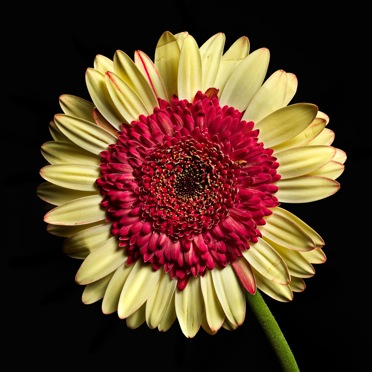
\includegraphics[scale=0.21]{img/originalFlower}}
     \subfigure[Edges]{\label{lssample}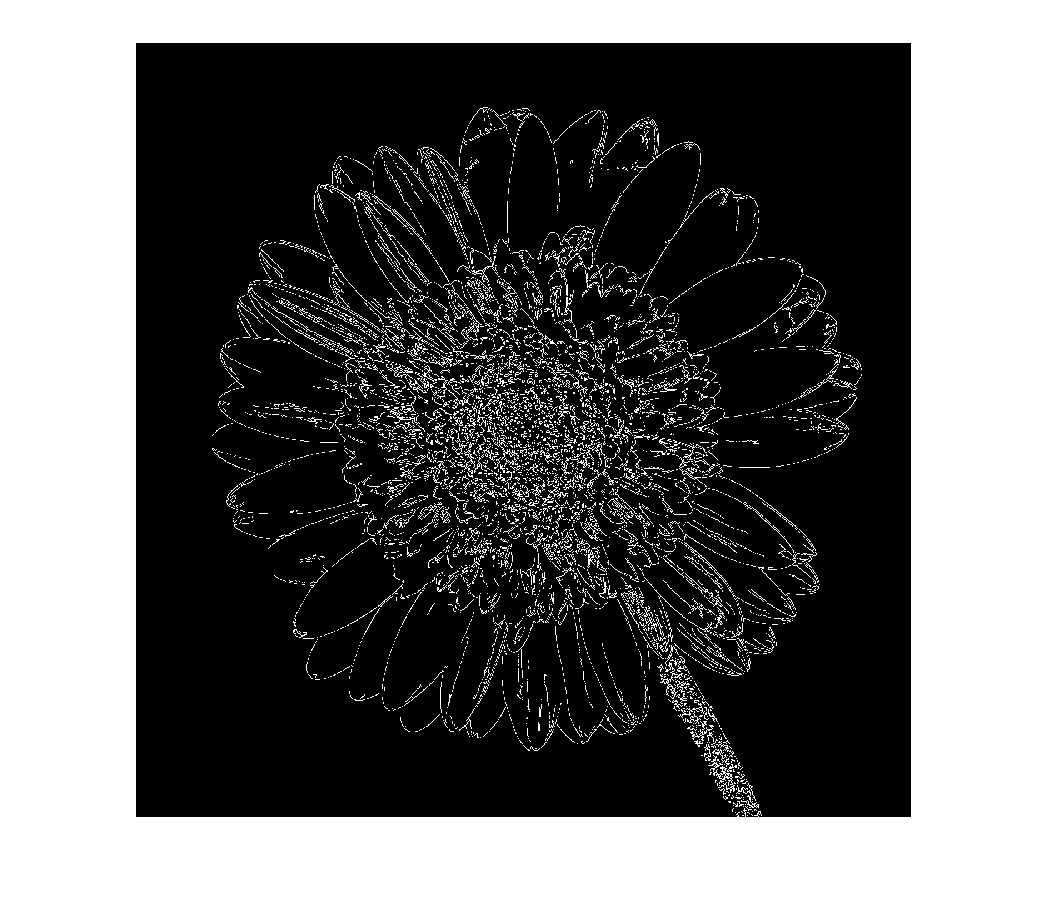
\includegraphics[scale=0.21]{img/edgesFlower}} 
     \subfigure[3x3 Grid for compositional edge-pixel ratio]{\label{gridExample}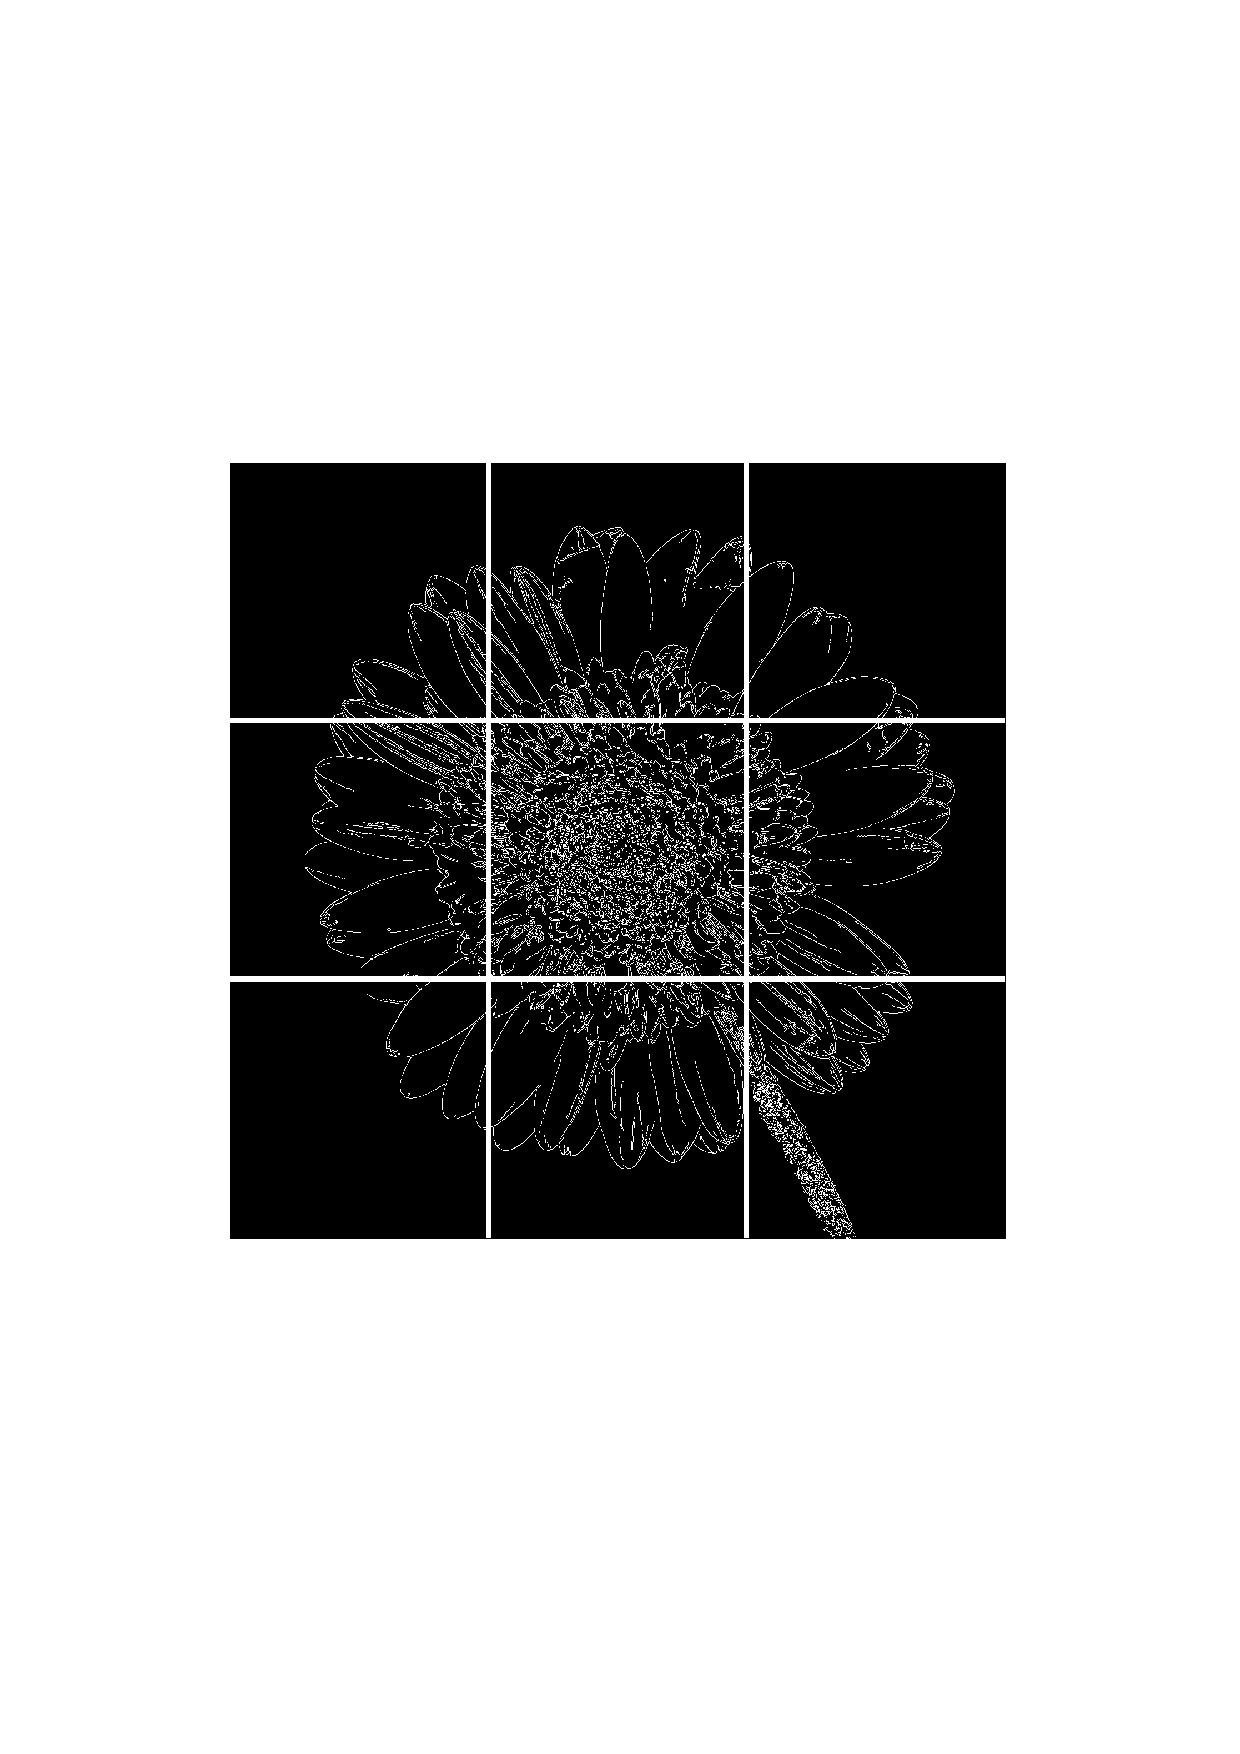
\includegraphics[scale=0.21]{img/gridEdgesFlower}}
     \subfigure[Corners]{\label{lssample}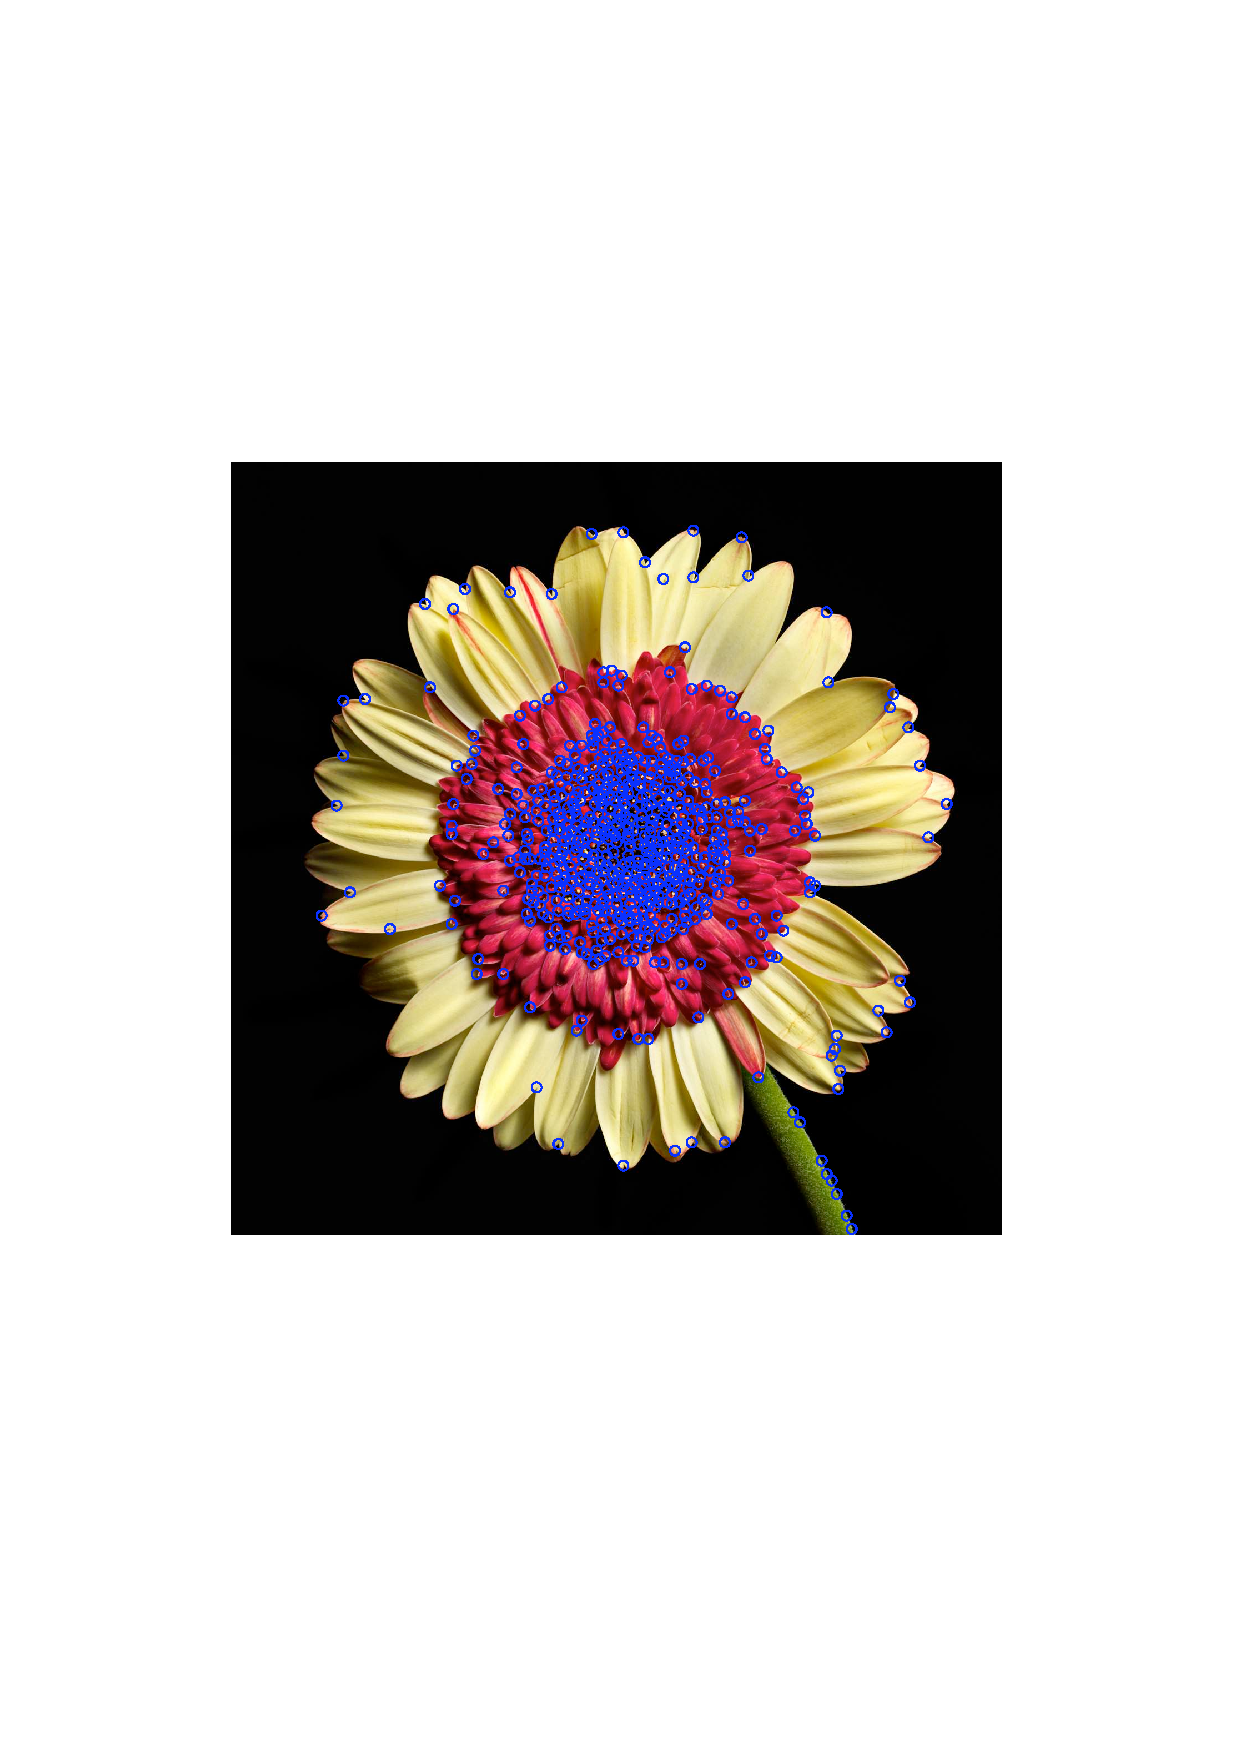
\includegraphics[scale=0.22]{img/cornersFlower}}  
     \subfigure[Hue]{\label{lssample}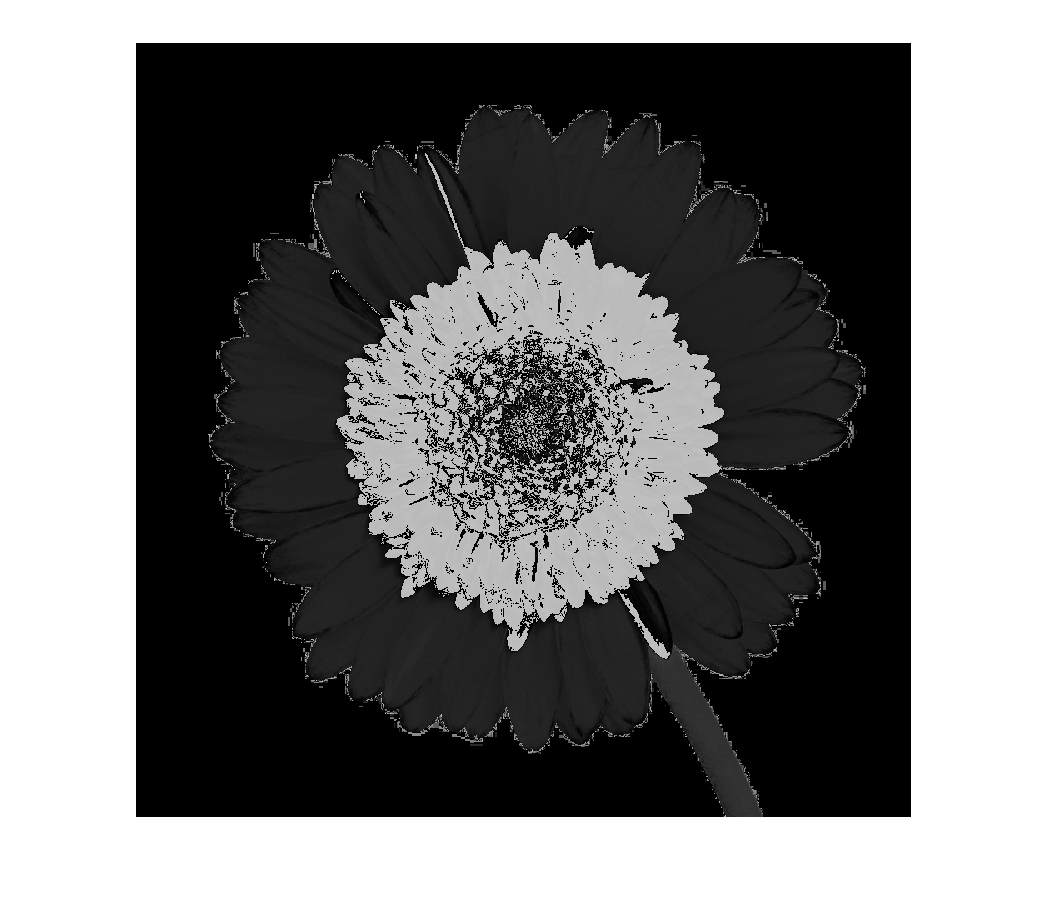
\includegraphics[scale=0.22]{img/hueFlower}}           
     \subfigure[Saturation]{\label{lssample}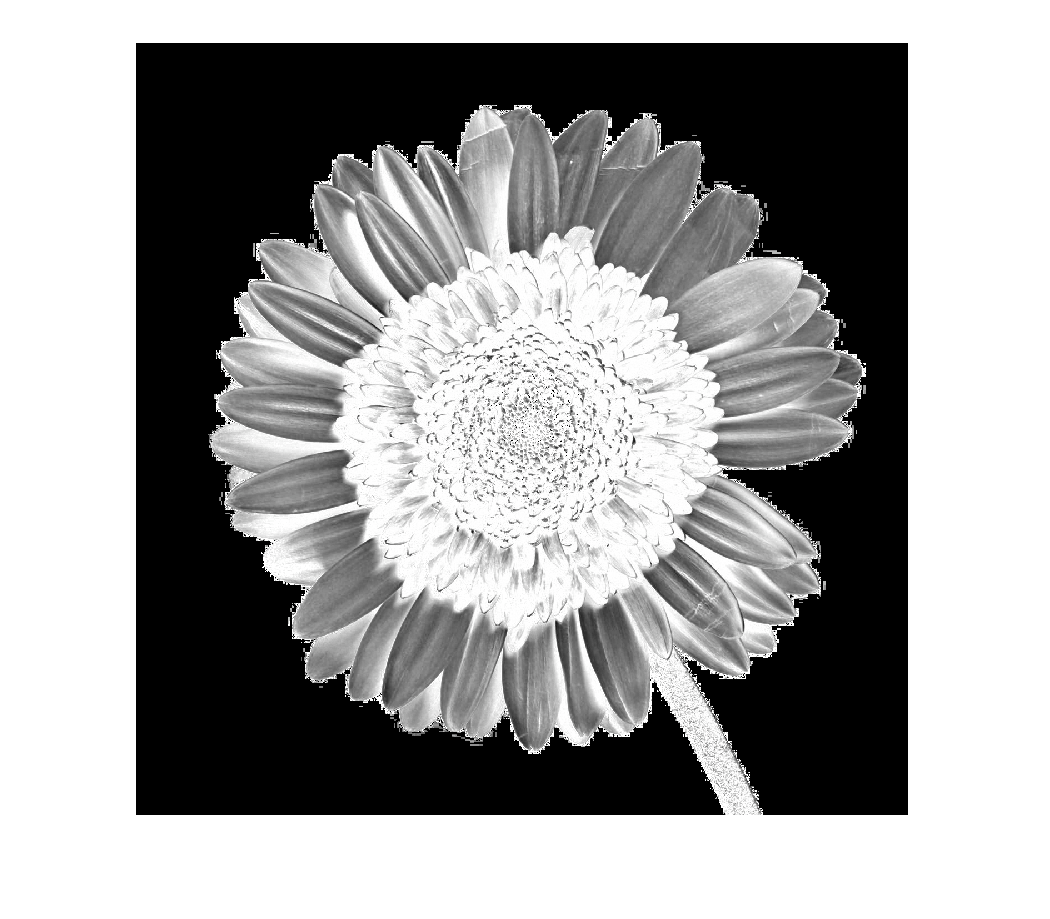
\includegraphics[scale=0.22]{img/satFlower}}           
     \subfigure[Value]{\label{lssample}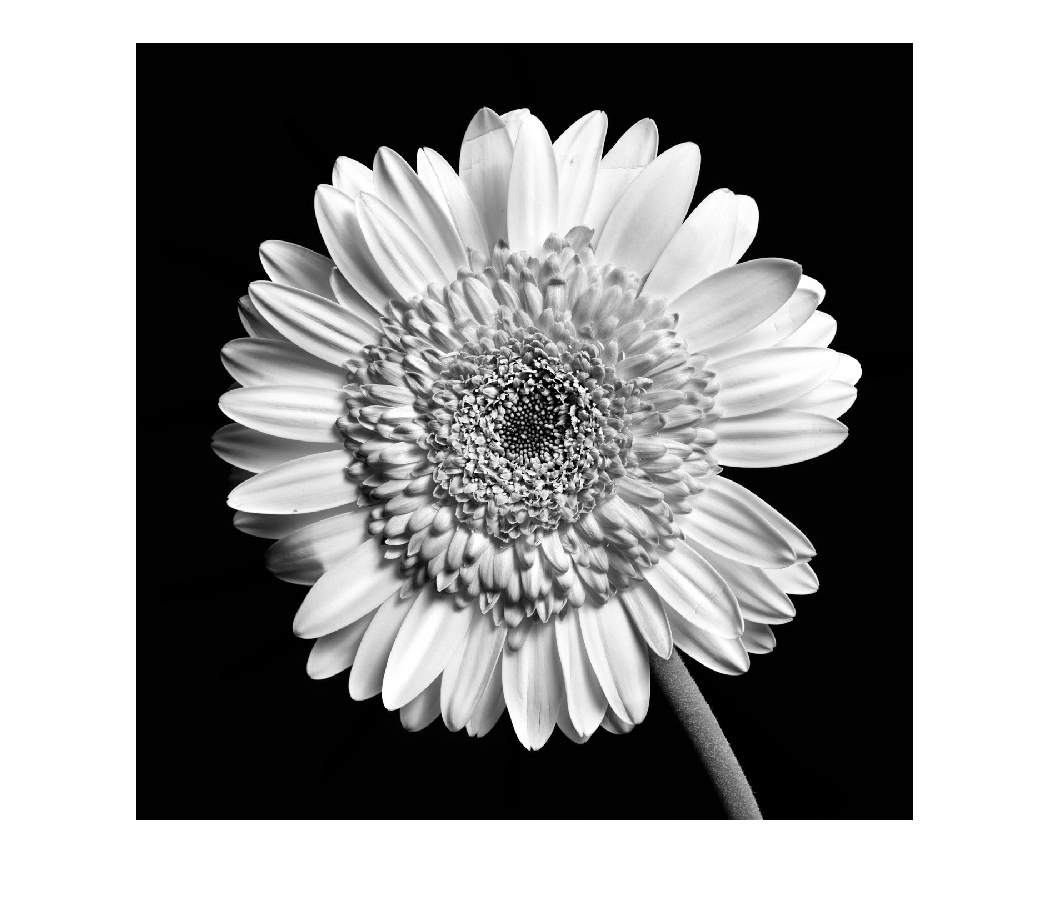
\includegraphics[scale=0.22]{img/valueFlower}}
     \subfigure[Intensity]{\label{lssample}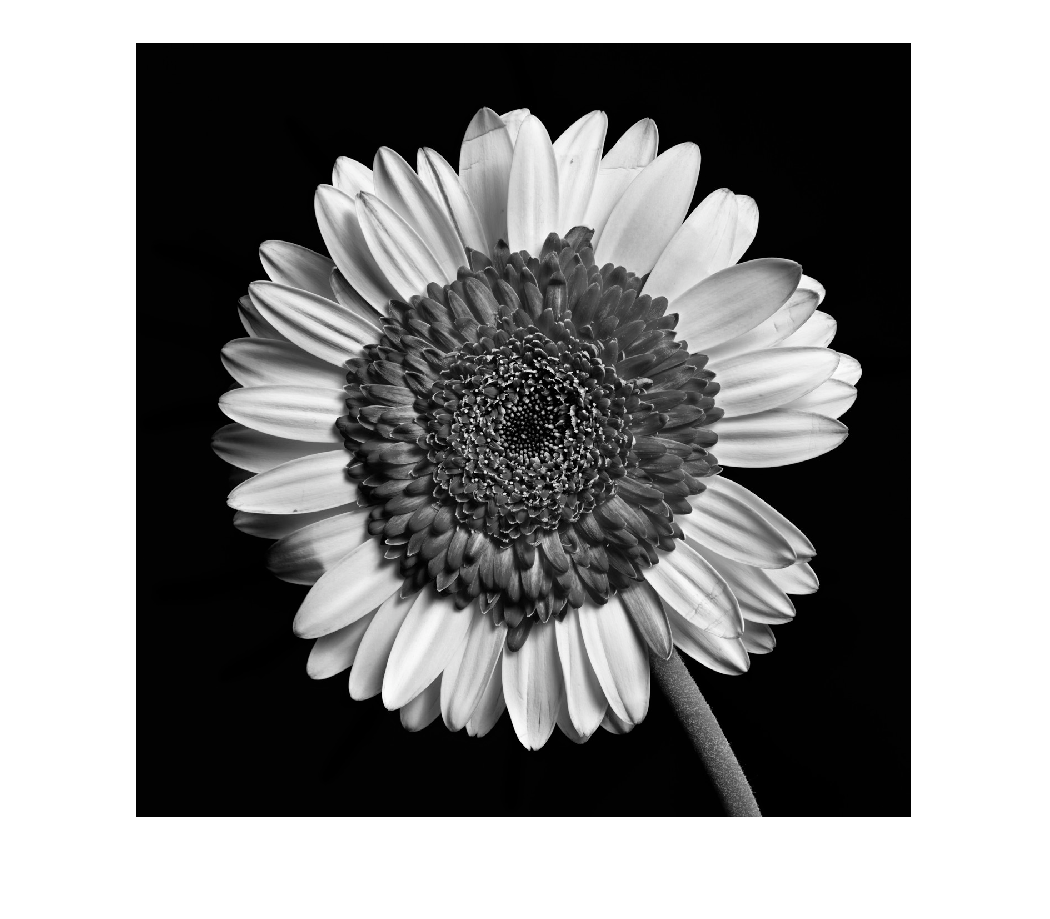
\includegraphics[scale=0.22]{img/intFlower}}                               
     \subfigure[Red]{\label{lssample}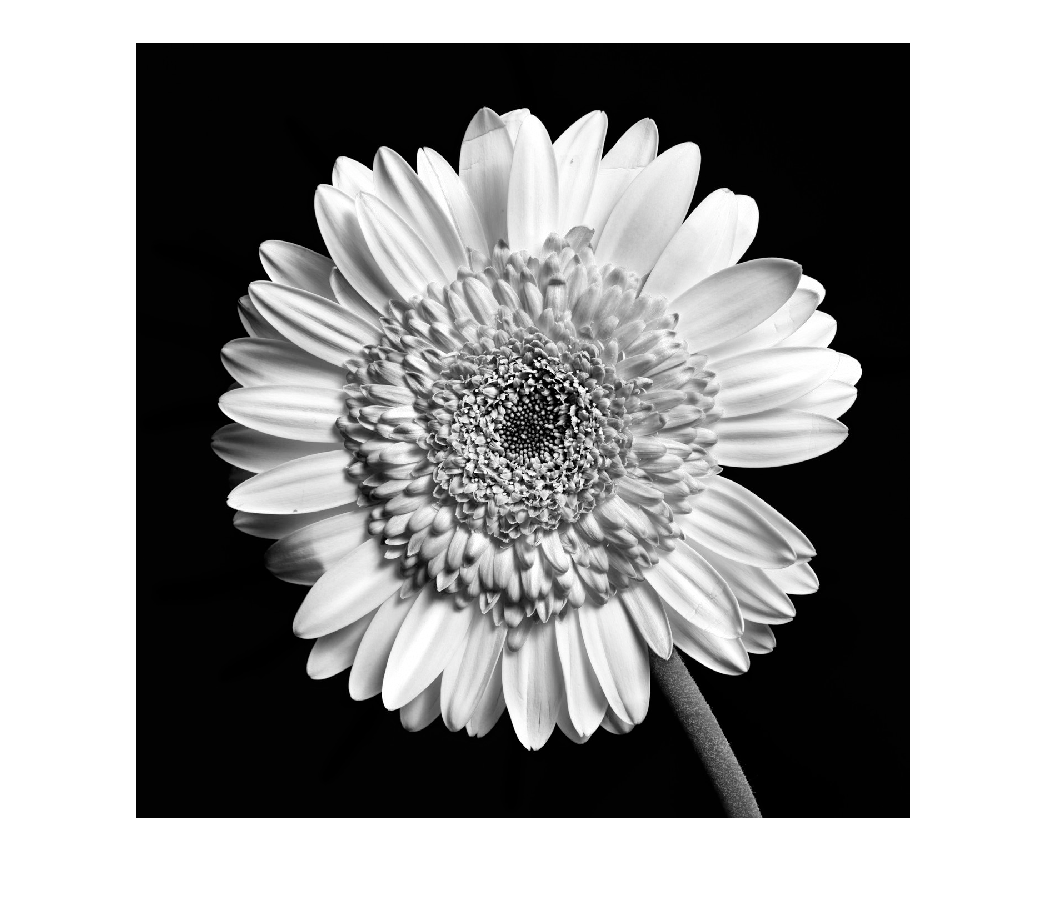
\includegraphics[scale=0.22]{img/redFlower}}
     \subfigure[Green]{\label{lssample}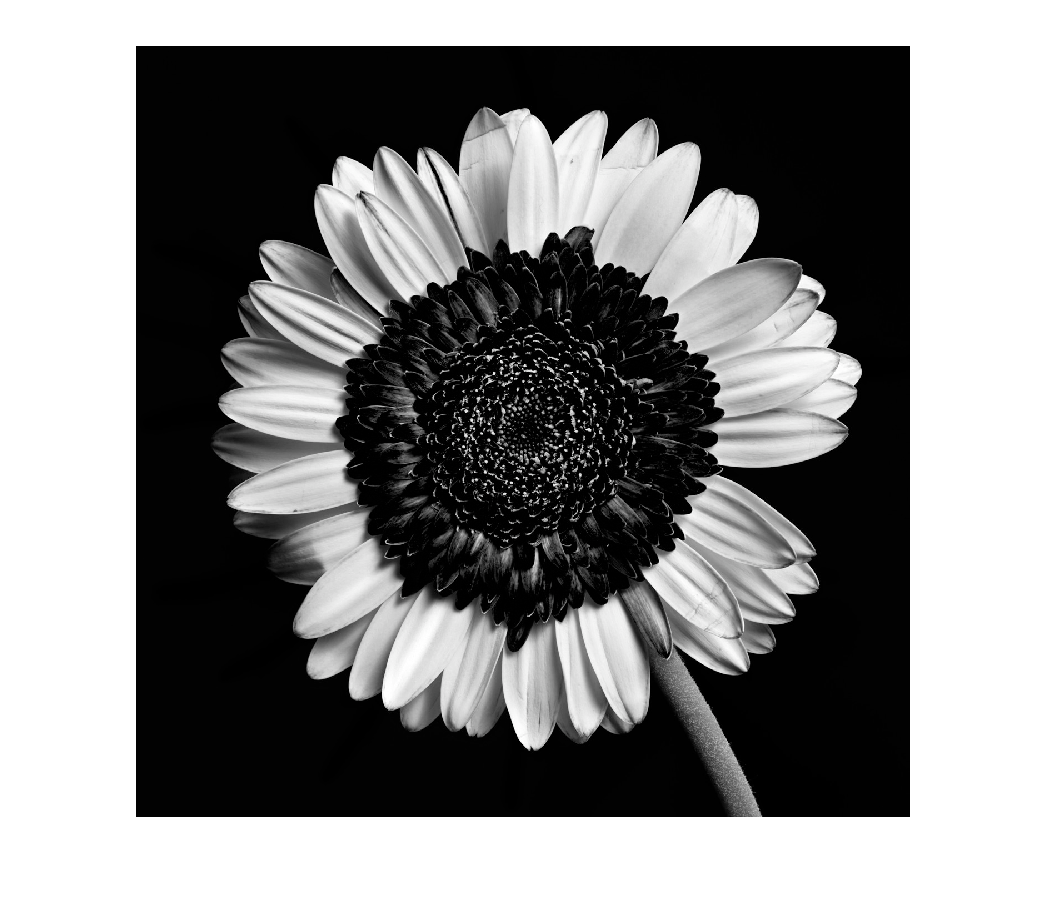
\includegraphics[scale=0.22]{img/greenFlower}}
     \subfigure[Blue]{\label{lssample}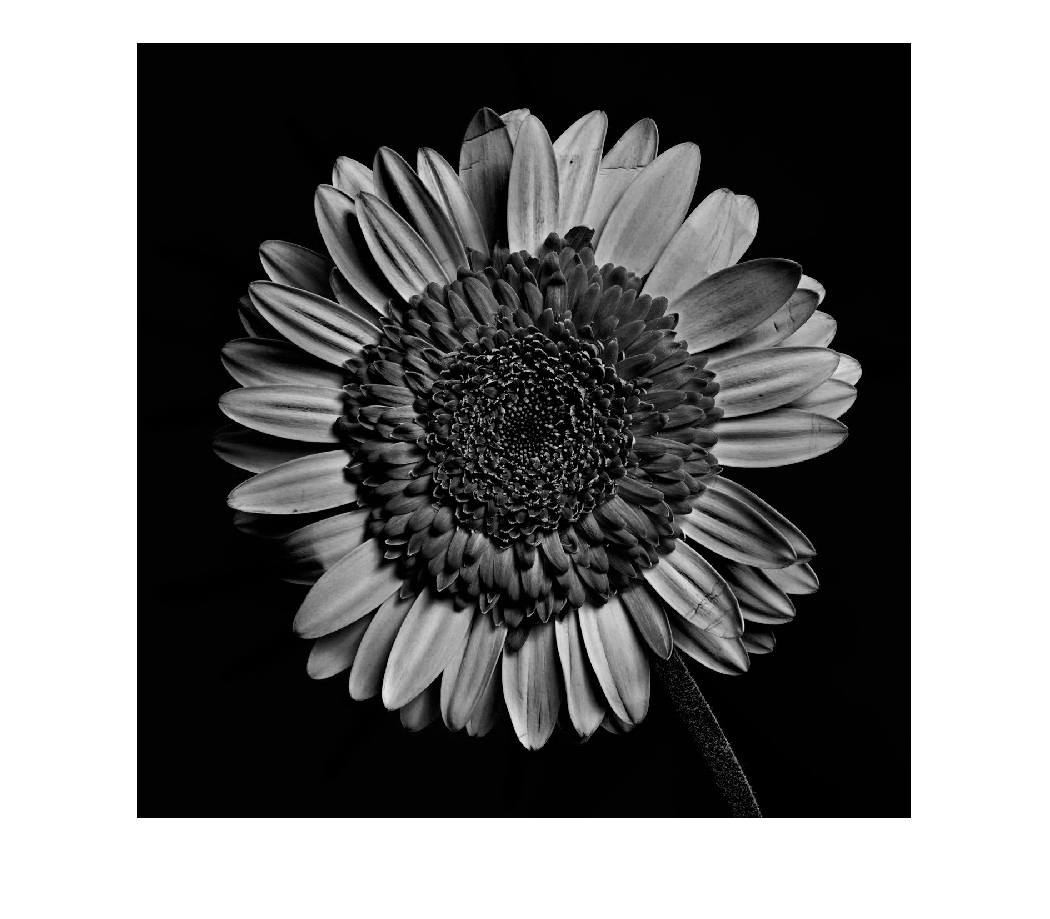
\includegraphics[scale=0.22]{img/blueFlower}}
   
  \end{center}
  \caption{Illustration of different statistical features}
  \label{featureImg}
\end{figure}


The features described so far only contain global information about images. In order to capture localized information as well, some of the features described above are also extracted from different regions of the image. The regions of the image are obtained by dividing the image along both dimensions into $NxM$ equal-sized regions. Since feature values will most likely vary from region region, these compositional features should provide valuable additional information about an image. Figure \ref{gridExample} shows an example of localized edge-pixel ratios using 3x3 equal-sized regions.\\ 

\paragraph{\textit{Cognitively-inspired features}\label{proposed-cognitive}}
A recent trend in computer vision research in the pursuit of human-like capability is the coupling of cognition and vision into cognitive computer vision. Cognitive computer vision has been introduced with the aim of achieving more robust, resilient, and adaptive computer vision systems by endowing them with a cognitive faculty.
%the ability to learn, adapt, weigh alternative solutions, and develop new strategies for analysis and interpretation.

Recent studies have focused on computational models of focal visual attention. Attention has been proven to influence the processing of visual information even in the earliest areas of primate visual cortex. Even more, it has been discovered that the interaction of bottom-up sensory information and top-down attentional influences create an integrated \textit{saliency map}, that can be defined as a topographic representation of relative stimulus strength and behavioral relevance across visual space \cite{Saliency_WWHW}. This map enables the visual system to integrate large amounts of information because it provides an efficient coding scheme for the potentially most relevant information in the sensory input. 
%, even from outside the fovea 
An important model based on this theory is provided by Itti, Koch and Niebur \cite{Itti_review,Itti_model}. Despite its simple architecture the model is capable of mimicking the properties of primate early vision on complex natural scenes.
The model works as follow: an input image is decomposed through several pre-attentive feature detection mechanisms which operate in parallel channels over the entire visual scene, and four conspicuity maps (color, orientation, intensity and skin) are created. After different intermediate steps, the model finally combines the four conspicuity maps into an unique saliency map. 

Until now the saliency map have been used as information channel in scene understanding and object recognition. In this research, image features are extracted from the map and used in the classification and visualization task. The features that have been extracted from those maps are: \textit{Shannon entropy} of the five maps, \textit{Standard deviation} of the distribution of attention in the saliency map, \textit{Location} of the most salient points (defined as the centers of the most salient regions) and \textit{Skin intensity} of the skin map. Skin is not a default channel in the Itti's model, but it has been found to be really interesting and useful in dA to distinguish artists and artworks, because there is a major presence of photographers that create nude art. 

\begin{figure}[h!]
\centering
\subfigure[]{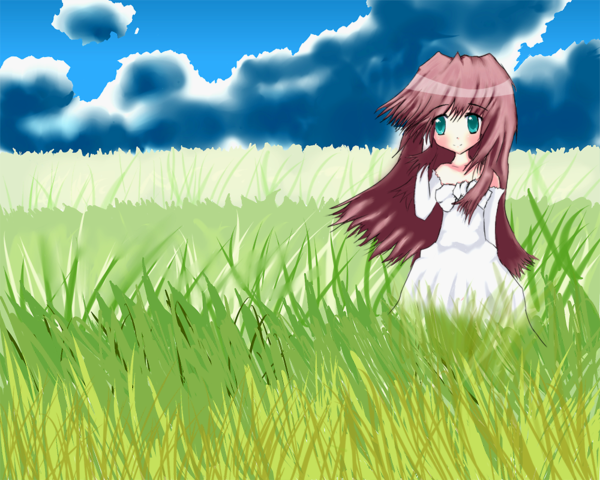
\includegraphics[scale=0.135]{Saliency_images/A_landscape_pic_with_a_loli_bg_by_CroireIgeen.png}\label{fig:saliencyimg1}}
\subfigure[]{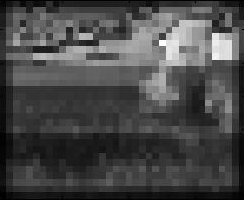
\includegraphics[scale=0.33]{Saliency_images/color.PNG}\label{fig:saliencyimgc1}}
\subfigure[]{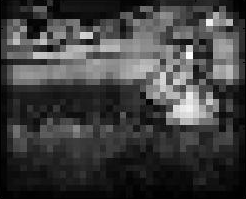
\includegraphics[scale=0.33]{Saliency_images/intensity.PNG}\label{fig:saliencyimgc2}}
\subfigure[]{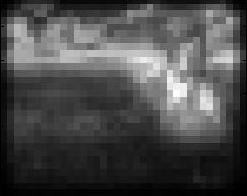
\includegraphics[scale=0.33]{Saliency_images/orientation.PNG}\label{fig:saliencyimgc3}}
\subfigure[]{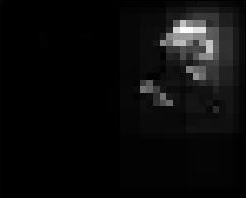
\includegraphics[scale=0.33]{Saliency_images/skin.PNG}\label{fig:saliencyimgc4}}
\subfigure[]{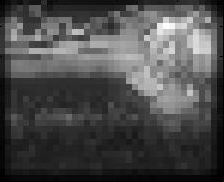
\includegraphics[scale=0.36]{Saliency_images/sm.PNG}\label{fig:ex_saliencymap}}

\caption{Example saliency maps. (f) shows the final saliency map, while (b), (c), (d) and (e) show the conspicuity maps for color, intensity, orientation and skin respectively.}
\end{figure}


\subsubsection{Classification}

An important aspect of this project is the description of images, artists or categories using the features that were extracted.
In this approach, classifiers are used to give a performance score to a set of features that is used to either describe an artist or a category.\\

\paragraph{\textit{Data normalization}}

Classifiers improve their performance when the dataset is normalized.
The extracted features have different value ranges, therefore it is important to rescale all the different ranges to a predefined one.

\begin{equation}
\label{minmax}
y_n=\frac{x_n - \max(x_n)}{\max(x_n)-\min(x_n)} * (B-A)
\end{equation}

Equation \ref{minmax} shows the \textit{Min/Max normalization} used to normalize the data.
In this equation [$A, B$] represent the predefined range; $x_n$ represents the unnormalized values of feature $n$ and $y_n$ represents the normalized ones.\\

\paragraph{\textit{Classifiers}}
Four different classifiers were incorporated to calculate the performance of a set of features.
All classifiers were chosen based on their expected performance.% except for the Nearest Mean classifier.

\textit{k-Nearest Neighbour}~\cite{korn1996fast} classifies an artwork based on the training examples that are close to it.
The Euclidian distance is used to measure the distance between a training sample and the artwork.

\textit{Naive Bayes}~\cite{keren2003recognizing} divides the value range for each feature in $n$ bins.
Then it counts the frequency of a training example for each of the classes in every bin and uses that to classify an artwork belonging to the class that gives the maximum posterior probability.

\textit{Nearest Mean} classifies an artwork based on the Euclidian distance to the mean of a class.
The classifier was chosen because it is a simple model.
%This is because the appropriate features of a class will make the artwork separable.

\textit{Support Vector Machine}~\cite{chapelle1999svms} classifies an artwork using a model learned from training examples.
The model represents the training examples by a decision boundary that separates the two classes by maximizing the distance to the decision boundary.
%The artwork is classified by the model based on which side of the decision boundary they fall on.\\

\paragraph{\textit{Feature selection}}
The classifiers are used to compute the performance score of a set of features.
Moreover a feature selection algorithm is used to extract a set of features out of all the features that were pre-computed.
This is intended to retrieve the smallest set of appropriate features to describe a class.

The feature selection starts by selecting the most informative feature and for each step iteratively adds the next most informative feature to it in a greedy fashion.

\begin{equation}
\label{featureselect}
F := F \cup f, where f: \max{J(f_i)} \wedge f_i \epsilon F
\end{equation}
Formula \ref{featureselect} represents this algorithm.
In this formula, $F$ represents the entire feature set, $f$ one single feature and $J$ the criterion that is used to define if a feature is informative.

The \textit{inter-intra distance} is used as the criterion to define if a feature is informative.
It works by measuring the inner-scatter of a class over a feature and measures it against the scatter of that class around the average of the feature.
For a two class problem the inter-intra distance can be written as:

\begin{equation}
\label{interintra}
J = \frac{|m_1-m_2|}{\sqrt(s^2_1 + s^2_2)}
\end{equation}
Here $m_1$ and $m_2$ are the average mean of class 1 and class 2, $s_1$ and $s_2$ are the standard deviations of those classes.
This equation is  equivalent to the Fisher criterion~\cite{malina1981extended}.\\

\paragraph{\textit{Evaluation measures}}
An evaluation measure is needed to measure the performance of the classifiers.
Every prediction of the classifier is labeled as one of the following four types,
depending on whether or not the classification was correct. This results in the confusion matrix:\\

\begin{tabular}{r|c|c|}
\multicolumn{1}{r}{}
 &  \multicolumn{1}{c}{predicted positive}
 & \multicolumn{1}{c}{predicted negative} \\
\cline{2-3}
positive & \textbf{tp} (true positive) & \textbf{fp} (false positive) \\
\cline{2-3}
negative & \textbf{fn} (false negative) & \textbf{tn} (true negative) \\
\cline{2-3}
\end{tabular}\\\\

With these standard classification measures two more evaluation measures can be computed.
These are precision and recall.
$Precision$ is defined as the number of relevant artwork correctly classified as positive divided by the total number of positive classified artwork.

\begin{equation}
Precision = \frac{tp}{tp + fp}
\end{equation}

$Recall$ is defined as the number of relevant artwork correctly classified as positive divided by the total number of positive examples in the dataset.

\begin{equation}
Recall = \frac{tp}{tp + fn}
\end{equation}

Precision and recall are then used to compute the $F-measure$.
This measure is the weighted harmonic mean of the precision and recall and can be defined as:

\begin{equation}
F_\beta = \frac{(1+\beta)^2 (Precision * Recall)}{(\beta ^2 * Precision) + Recall}
\end{equation}

$\beta$=1 has been used, which means that precision and recall are evenly weighted.